%%%%% Template for MTH 227 Daily Assignments 


\documentclass[11pt]{article}

\pagestyle{empty}                       %no page numbers
\thispagestyle{empty}                   %removes first page number
\setlength{\parindent}{0in}               %no paragraph indents

\usepackage{fullpage}
\usepackage[tmargin = 0.5in, bmargin = 1in, hmargin = 1in]{geometry}     %1-inch margins
\geometry{letterpaper}                  
\usepackage{graphicx}
\usepackage{amssymb}

% Default packages
\usepackage{latexsym}
\usepackage{amsfonts}
\usepackage{amsmath}
\usepackage{amsthm}
\usepackage{palatino}
\usepackage{hyperref}
\usepackage{multicol}
\usepackage{fancyhdr}
\usepackage{enumitem}


\begin{document}
	
	
	\vspace*{0in}

		\begin{center}
			\begin{large}
			MTH 201: Calculus \\
			\textbf{Guidelines for Style and Formatting for Portfolio Problems} \\
			\end{large}
		\end{center}
		
This document gives basic guidelines for writing up solutions to Portfolio Problems. We reserve the right to add more guidelines to the list if new issues arise. 
		
\section*{Solution Style and Formatting}

When writing up your solutions to Portfolio problems, make sure you are attending to each of the following\footnote{Most of these items are taken from \emph{Mathematical Reasoning: Writing and Proof} by Theodore Sundstrom, the textbook used in MTH 210: Communicating in Mathematics.}: 

\begin{itemize}
	\item Your audience for Portfolio Problems will always be \textbf{a peer in MTH 201 who is knowledgeable in all the calculus content that we have covered in the class but who is unfamiliar with the specific problem you are solving}. Every solution you write is to be an attempt to persuade such a person that your solution is correct. 
	\item Begin each solution with a carefully-worded statement of the problem you are solving. 
	\item If you introduce a variable that represents a certain quantity, state explicitly what the variable represents when you introduce it. 
	\item Before doing any calculations, explain to the reader what you are about to do. For example, if you need to find the roots of the polynomial $3x^2 + x - 1$, then first say: ``We will use the Quadratic Formula to find the roots'' before doing the calculation. 
	\item Use the pronoun ``we'' instead of ``I''. For example: ``We will use the Quadratic Formula to find the roots'' and not ``I will use the Quadratic Formula to find the roots''. 
	\item Keep the reader informed of what you are doing at all times. Examples: 
	\begin{itemize}
		\item We will find the critical values of $p$ by solving the equation $p' = 0$. [\emph{Then solve the equation.}]
		\item We will first calculate the first and second derivatives of $f$. 
		\item We use the limit definition of the derivative to set up the following limit... 
	\end{itemize}
	\item Tell the reader when the solution has been completed. 
	\item Always include units on your answers if units are involved in the problem. 
	\item When working a problem with multiple parts, write solutions separately for each part and do not make one large writeup that encompasses all the parts. 
	
	
\end{itemize}


\section*{English Grammar and Usage}

Students in MTH 201 are expected to use correct and clear English when doing any writing. In some contexts in the class, informal use of English is acceptable, but for Portolio Problems the expectation is that the major rules for English usage are followed. We will adopt the following subset of English grammar and usage rules for MTH 201 portfolio problems. 

\begin{itemize}
	\item Use complete sentences, capitalizing the beginning word of each sentence and ending each sentence with an appropriate punctuation mark. 
	\item All words must be spelled correctly. 
	\item Never use slang, and avoid using abbreviations unless context suggests that this is acceptable. (For example ``DNA'' is preferable to ``deoxyribonucleic acid'', but ``critical value'' is preferable to ``c.v.''. )
	\item Special case of the previous point: The term ``plug in'' is slang and should never be used in a formal writeup. (It's OK for informal communication, just not formal.) Use the term ``evaluate'' instead. 
		\begin{itemize}
			\item \emph{WRONG}: We plug in $x = 5$ into the expression. 
			\item \emph{RIGHT}: We evaluate the expression at $x=5$. 
		\end{itemize}
	
	
	\item Subjects must agree with verbs. 
	\begin{itemize}
		\item \emph{WRONG}: The inflection points of this function lies in the interval $[1,3]$. 
		\item \emph{RIGHT}: The inflection points of this function lie in the interval $[1,3]$. 
	\end{itemize}
	
	\item The pronoun ``it'' must be used with care; the thing to which the ``it'' is referring must be clear from context. When in doubt, do not use a pronoun. 
	\begin{itemize}
		\item \emph{WRONG}: Since it is positive, it is increasing. 
		\item \emph{WRONG}: Since the derivative of $f$ is positive, it is increasing. [\emph{Still don't know what ``it'' is}]
		\item \emph{RIGHT}: Since $f'$ is positive, $f$ is increasing. 
	\end{itemize}
	
	\item Do not mix mathematical notation with English. 
	\begin{itemize}
		\item \emph{WRONG}: We now see that the left side = the right side. 
		\item \emph{RIGHT}: We now see that the left side equals the right side. 
	\end{itemize}
	
	\item Do not start a sentence with a variable. Avoid starting sentences with numbers; but if this cannot be avoided, spell the number out completely. 
	\begin{itemize}
		\item \emph{WRONG}: $c$ represents the parameter in this family of functions. 
		\item \emph{RIGHT}: Denote the parameter in this family of functions by $c$. 
	\end{itemize}
	
	
\end{itemize}


\section*{Formatting Mathematics}

\begin{itemize}
	
	\item Use italics for variables and regular, non-italicized fonts for the names of the trigonometric and logarithmic functions. 
	\begin{itemize}
		\item \emph{WRONG}: Suppose f(x) is a continuous function. 
		\item \emph{RIGHT}: Suppose $f(x)$ is a continuous function. 
		\item \emph{WRONG}: The derivative of $sin(x)$ is $cos(x)$. 
		\item \emph{RIGHT}: The derivative of $\sin(x)$ is $\cos(x)$. 
	\end{itemize}
	
	\item Do not use \verb=*= for multiplication or \verb=^= for exponents. Instead, use either a small dot or juxtaposition to indicate multiplication, and use superscripts to indicate exponents. 
	\begin{itemize}
		\item \emph{WRONG}: The derivative of \verb=x^2= is $2x$. 
		\item \emph{RIGHT}: The derivative of $x^2$ is $2x$. 
		\item \emph{WRONG}: We have that $A = l \ast w$ since the figure is a rectangle. 
		\item \emph{RIGHT}: We have that $A = lw$ since the figure is a rectangle. 
	\end{itemize}
	
	\item Always use parentheses to denote groups, and make sure parentheses match. 
		\begin{itemize}
			\item \emph{WRONG}: $x - x - 1 = 1$
			\item \emph{RIGHT}: $x - (x-1) = 1$
			\item \emph{WRONG}: $(x+1)(x-1 = x^2 - 1$
			\item \emph{RIGHT}: $(x+1)(x-1) = x^2 - 1$
		\end{itemize}
		
	\item Parentheses, square brackets, and other delimiters need to be of an appropriate size. 
		\begin{itemize}
			\item \emph{WRONG}: $\dfrac{d}{dx}[ \dfrac{x^2 - 1}{\tan(x)} ]$
			\item \emph{RIGHT}: $\dfrac{d}{dx}\left[ \dfrac{x^2 - 1}{\tan(x)} \right]$
		\end{itemize}
	
	\item Avoid using the “/“ symbol for complicated fractions. Use your word processor or typesetting language to make a multi-level fraction instead. 
	\begin{itemize}
		\item \emph{WRONG}: $2/(2 + 1/(2 + 1/2))$
		\item \emph{RIGHT}: $\frac{2}{2 + \frac{1}{2 + 1/2}}$
	\end{itemize}
	
	\item The equals sign ``='' is used only to claim that one expression truly equals another. \textbf{Any other use of the equals sign is incorrect.} 
	\begin{itemize}
		\item \emph{Example}: Using the equals sign to \emph{indicate a step in a calculation} is wrong: 
		\[ x^2 - 1 = 0 = (x-1)(x+1) = 0 = x = 1 \ \text{or} \, x = -1\]
		A correct alternative is to turn this into a narrative like so: 
		\begin{quote}
			Since $x^2 - 1 = 0$, we have $(x-1)(x+1) = 0$. From this we see that $x=1$ or $x = -1$.
		\end{quote}
		
		\item \emph{Example}: Using the equals sign to indicate a relationship between two expressions \emph{other than equality} is wrong, for instance: 
		\[ x^2 = 2x \]
		These two items are not equal! But the derivative of the left side equals the right side. This would be correctly phrased as: 
		\[ \frac{d}{dx}[x^2] = 2x \]
		
		\item \emph{Example}: Using the equals sign to denote \emph{approximate equality} is wrong. Use the ``approximately equals'' ($\approx$) symbol instead. 
			\begin{itemize}
				\item \emph{WRONG}: $1/3 = 0.333$  [\emph{These two are not exactly equal}]
				\item \emph{RIGHT}: $1/3 \approx 0.333$ 
				\item Also \emph{RIGHT}: $1/3 = 0.333\dots$ [\emph{The dots indicate that the pattern in the decimals continues forever}]
			\end{itemize}
		
	\end{itemize}
	
	\item Related to the previous point: The term \emph{equation} refers to a statement that two expressions are equal. Equations always consist of two mathematical expressions joined by the equals sign. \textbf{Anything else is not an equation and should not be referred to as an equation}. A single mathematical statement (for example, only the left side of an equation) is called an \emph{expression}. 
		\begin{itemize}
			\item \emph{WRONG}: The equation $x^2 - 1$ factors into $(x+1)(x-1)$. 
			\item \emph{RIGHT}: The expression $x^2 - 1$ factors into $(x+1)(x-1)$. 
			\item \emph{WRONG}: We now plug in $x=5$ to the equation $e^x$. 
			\item \emph{RIGHT}: We now evaluate the expression $e^x$ at $x=5$. [\emph{See the previous section about the phrase ``plug in''}]
		\end{itemize}
	
	
		
	\item Variable names must be used consistently. In particular, if a function or expression uses a particular letter for a variable, you may not simply relabel it as $x$, and if a function has a particular letter for its name you may not simply rename it as $f$. 
	\begin{itemize}
		\item \emph{WRONG}: $f(t) = x^2 - x + 1$  [\emph{Changed variable on the right side}]
		\item \emph{RIGHT}: $f(t) = t^2 - t + 1$
		\item \emph{WRONG}: Since $A(x) = x^2$, we know that $f'(x) = 2x$. [\emph{Changed function name}]
		\item \emph{RIGHT}: Since $A(x) = x^2$, we know that $A'(x) = 2x$. 
	\end{itemize}
		
	\item Important mathematical computations or expressions should be set off on a line by themselves and centered. If one side of a column of equations doesn't change, then it should not be repeated. For example: 
		\begin{align*}
			x &= \frac{-b \pm \sqrt{b^2 - 4ac}}{2a} \\
			  &= \frac{-1 \pm \sqrt{1^2 - 4 \cdot 3 \cdot (-1)}}{2 \cdot 3} \\
			 &= \frac{-1 \pm \sqrt{13}}{6}
		\end{align*}
		
	\item Use decimal approximations only when necessary or when context calls for it. Otherwise use exact values. If you are using decimal approximations, carry decimal approximations out to a length that is appropriate for the context but not too short. 
		\begin{itemize}
			\item WRONG: A circle with radius $1$ has a circumference of approximately $6.28$. [\emph{Context does not call for an approximation}]
			\item RIGHT: A circle with radius $1$ has a circumference of $2 \pi$. 
			\item WRONG: The total cost of lunch is \$5.681823. [\emph{Decimal is too long for the context of money}]
			\item RIGHT: The total cost of lunch is \$5.68. [\emph{Truncating to the hundreds place makes more sense here}]
			\item WRONG: A circle with radius of $2.11$ has an area of approximately $14$. [\emph{True, but too much roundoff}]
			\item RIGHT: A circle with radius of $2.11$ has an area of approximately $13.9867$. [Since the radius is given as a decimal, a good approximation is warranted by the context.]
			\item Also RIGHT:  A circle with radius of $2.11$ has an area of exactly $\pi \cdot (2.11)^2$. [\emph{True and exact; but perhaps the decimal approximation above is more informative.}]
		\end{itemize}
	
	\item When doing repeated calculations that involve the same work over and over again but on different inputs, it is sufficient to show complete work on one of those calculations and then only the setup and answer for the work on the rest (unless there is some reason in the problem for showing complete work on everything). 
			
	\item Clear English is better than cumbersome mathematical notation. When using notation that seems complex, try rephrasing in the form of an English sentence with minimal notation. Then use the version that makes the most sense to your reader. 
	
		
	\end{itemize}
	
	
	
\section*{Formatting Graphs}
When making a graph of a function, please use Geogebra, Wolfram\textbar Alpha, or some other mathematical software capable of creating professional-quality graphs. All graphs of functions should have these properties: 
\begin{itemize}
	\item The graph is situated in an appropriate viewing window with minimal dead space. For example, here are two graphs of $y = e^x$. The one on the left has too much unused dead space. The one on the right is better situated. 
	\begin{center}
		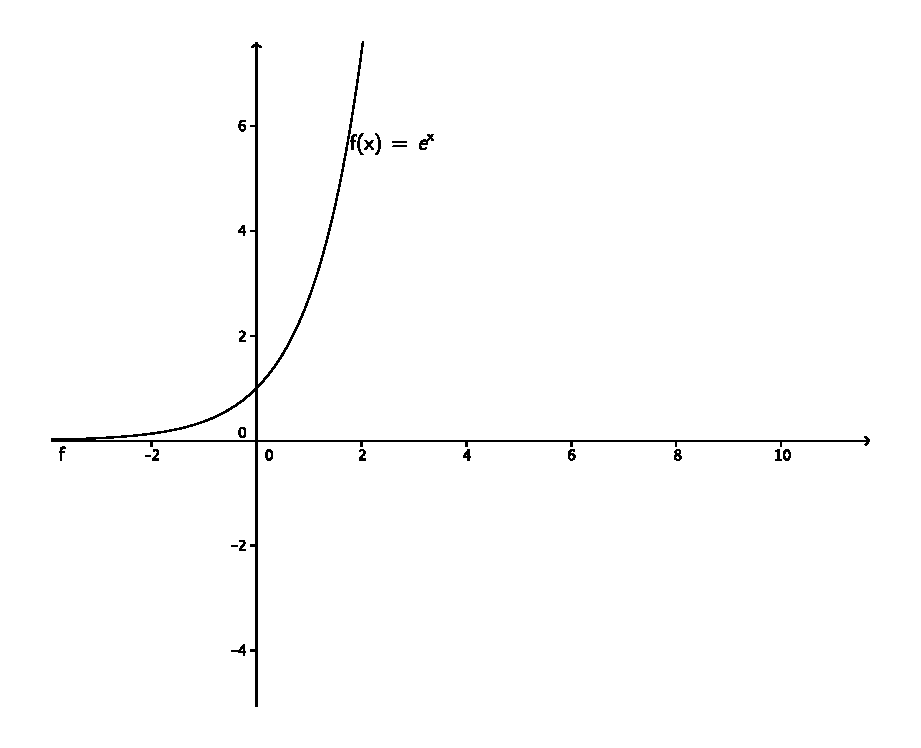
\includegraphics[width=2.5in]{badgraph1}
		\qquad
		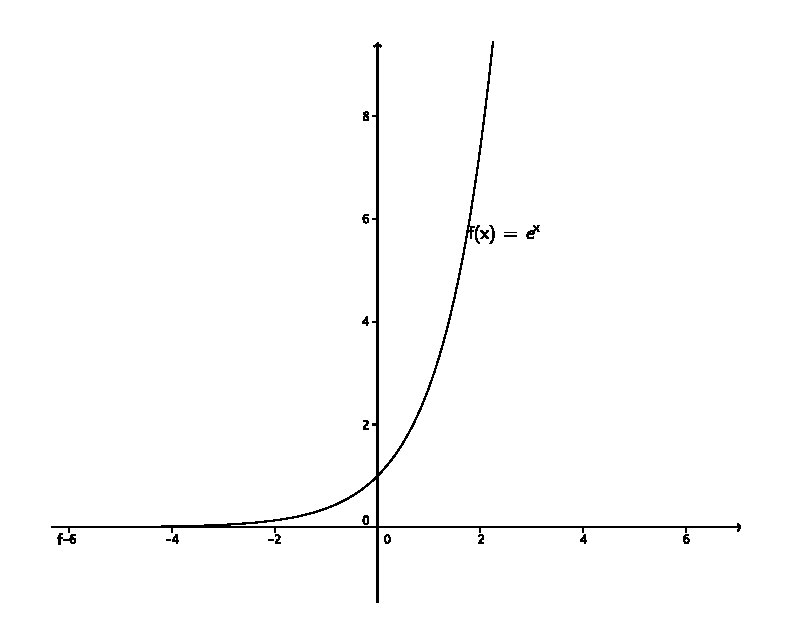
\includegraphics[width=2.5in]{goodgraph1}
	\end{center}
	
	\item \textbf{Both axes should be labelled clearly}. Three items of information should be included on each axis label unless that information is not available: \textbf{the quantity being represented, the symbol being used, and the units of measurement.} The quantity should be spelled out, the symbol should appear next in parentheses ( ), and then the units should appear next in square brackets [ ]. For example, if the formula $v = -4.9t^2 + 100$ represents the velocity (in meters per second) of a falling object at a given time (in seconds), then here's a proper plot of that formula (produced in Geogebra): 
	\begin{center}
		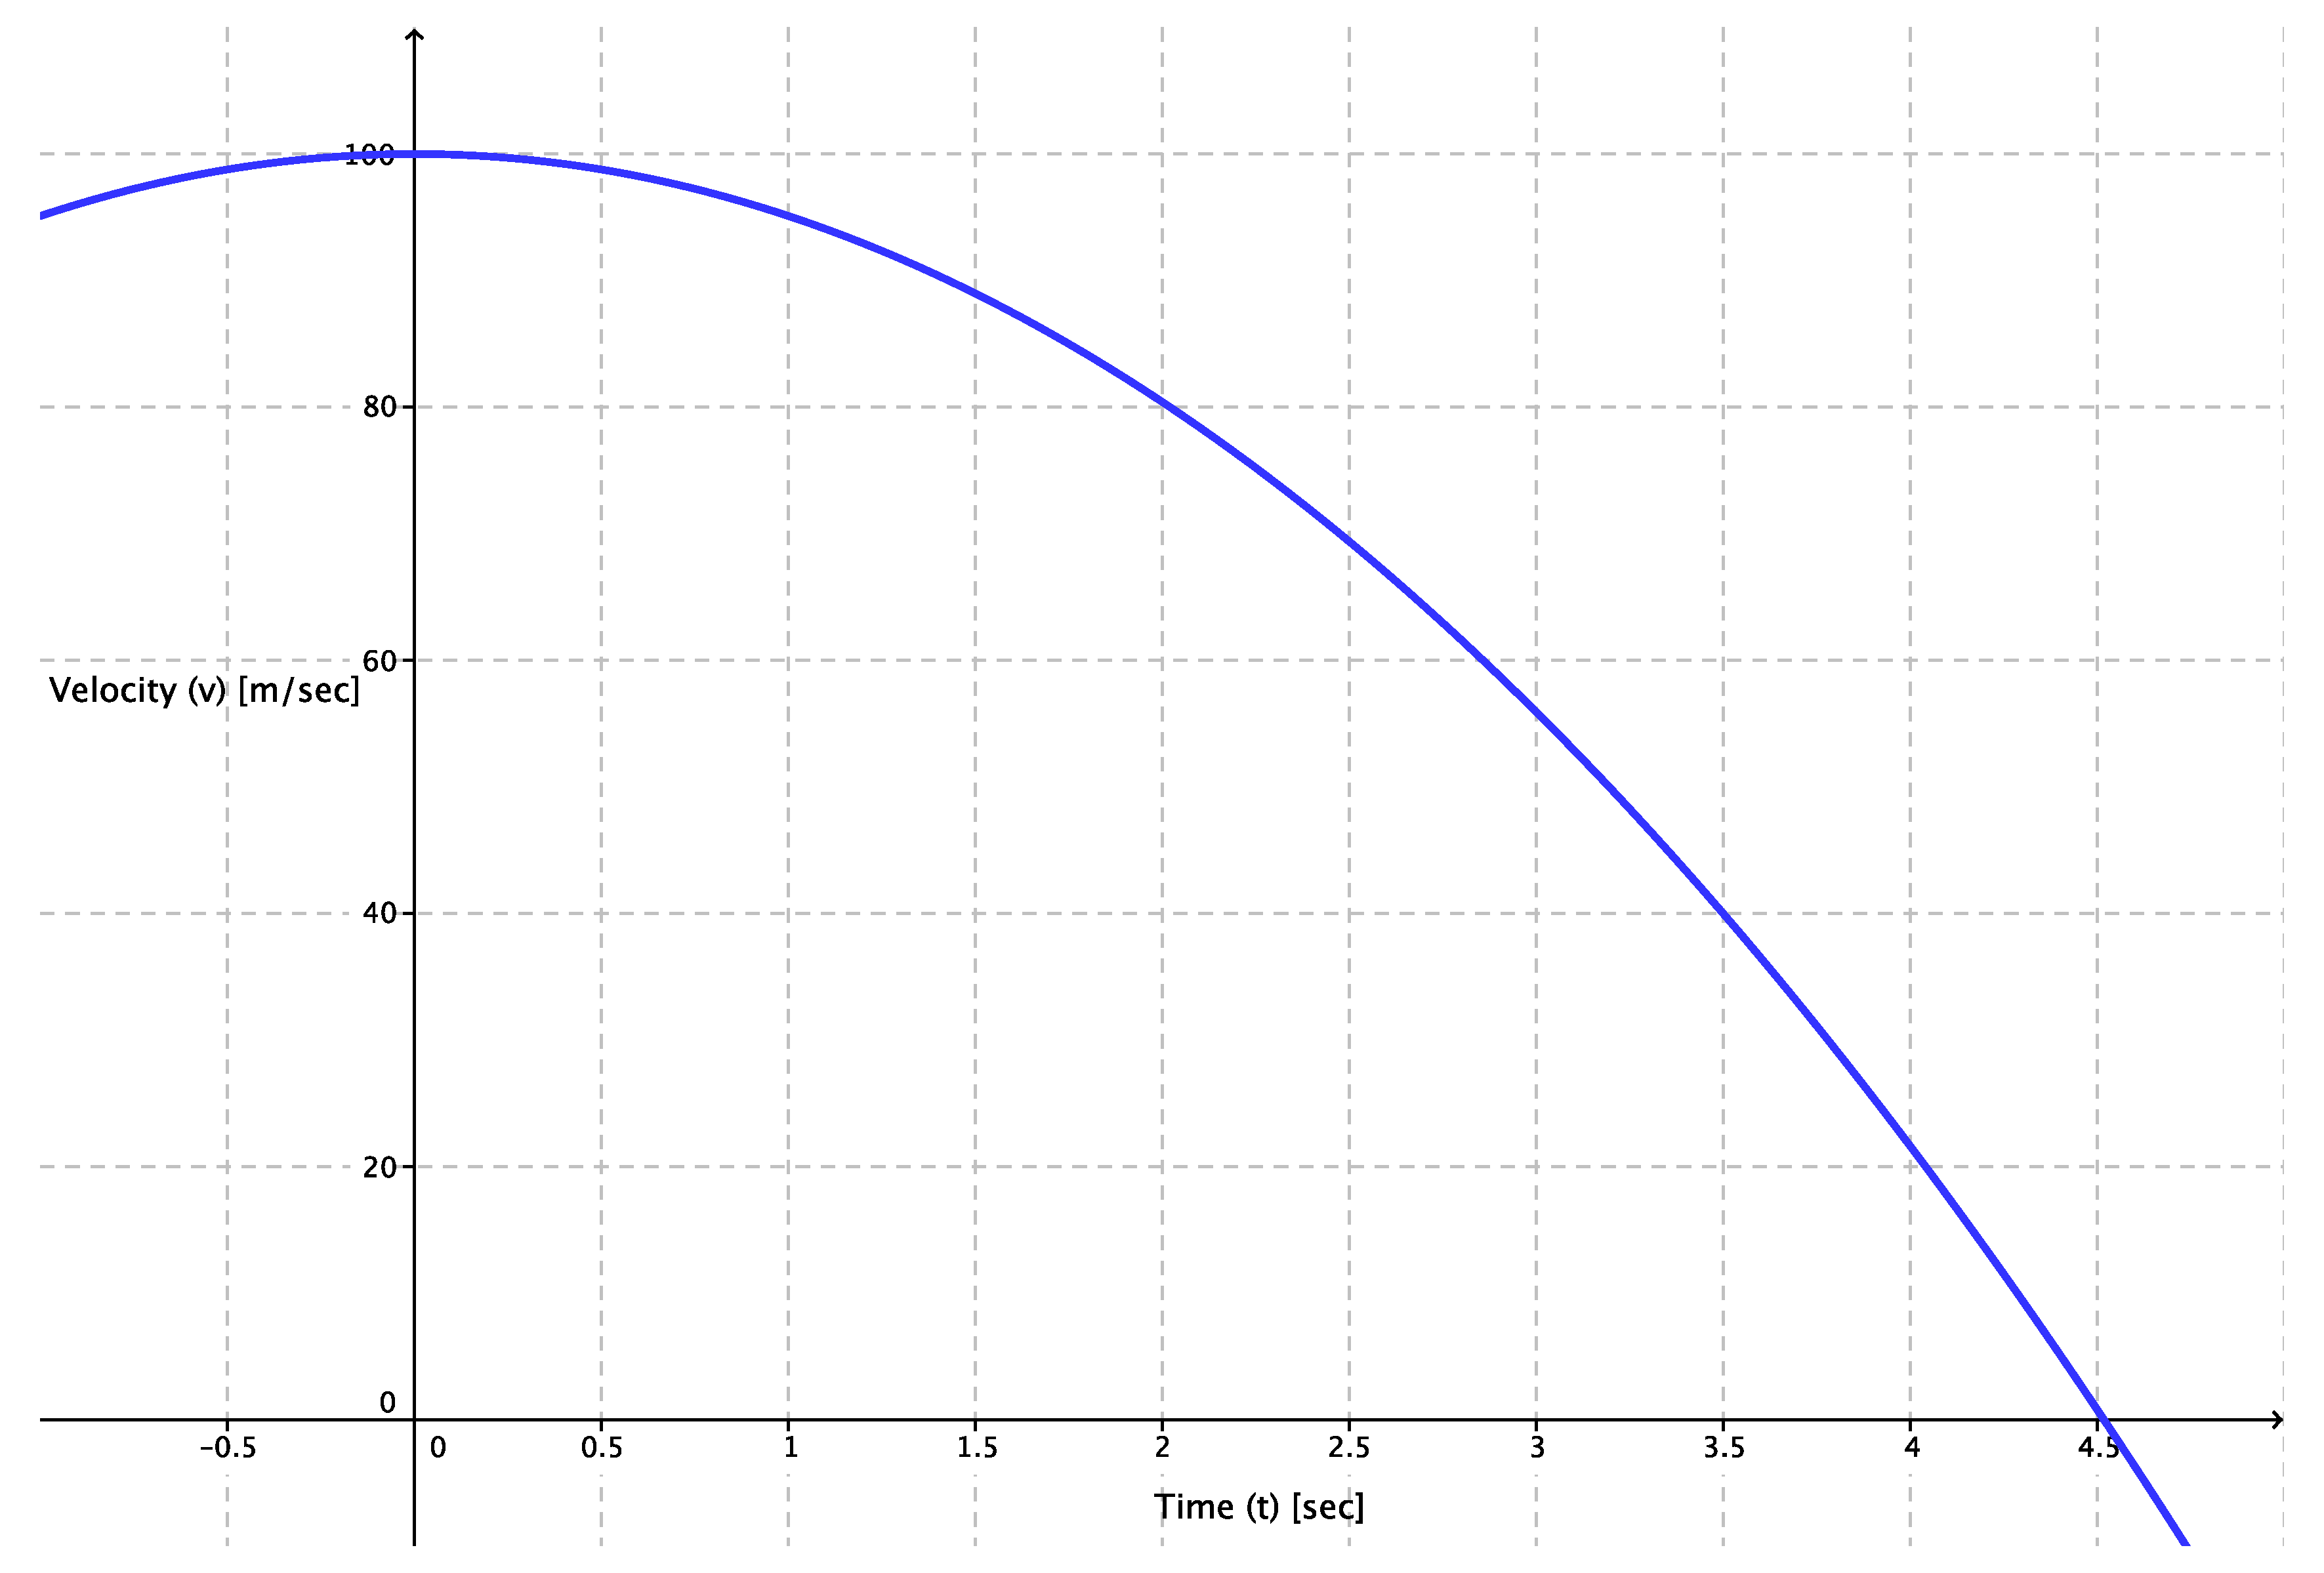
\includegraphics[width=3.5in]{properplot}
	\end{center}
	
	\item \textbf{Show scaling on both axes} unless your graph is just a conceptual sketch. Choose scale increments for both axes that are easy to read and interpolate betwee; avoid unusual or unnatural increments. For example, the plot above uses sensible increments of scaling (0.5 on the time axis, 20 on the velocity axis). 
	
	\item \textbf{Provide horizontal and vertical gridlines} to make interpolation easier, unless your graph is just a conceptual sketch. 
	
	\item If you are making a single plot with two or more graphs on it, use different colors for the different functions and, if possible, include a legend that makes it easy to tell the functions apart. For example, here are two different plots of the functions $f(x) = \sin(x)$ and $g(x) = \cos(x)$ (again, produced in Geogebra): 
	\begin{center}
		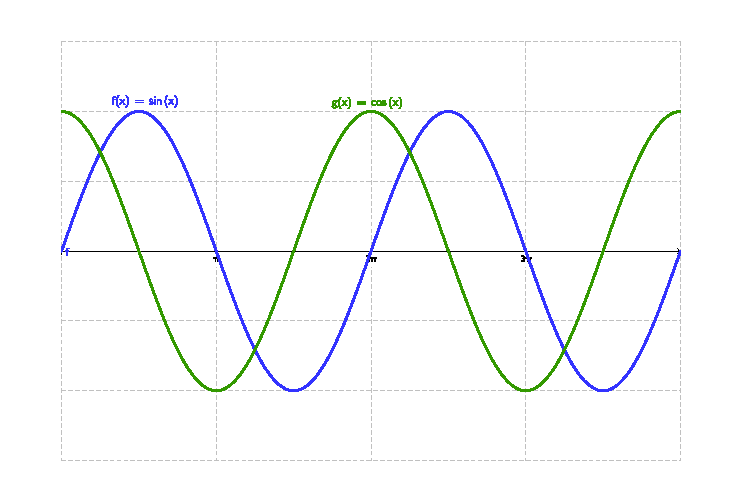
\includegraphics[width=2.7in]{twographs1}
		\qquad
		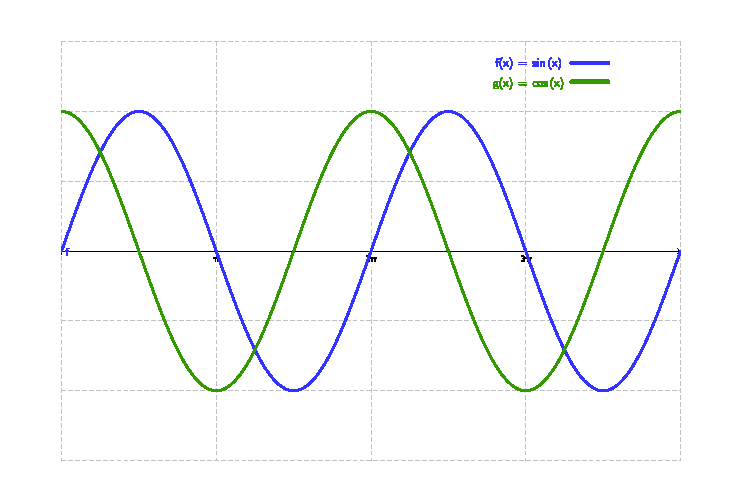
\includegraphics[width=2.7in]{twographs2}
	\end{center}
The plot on the left has the names of the functions attached directly to their graphs and done in matching colors. The plot on the right has a separate legend in the top-right corner that indicates which color is which function. Either way is acceptable. 
	
	
	
\end{itemize}

		
\section*{Formatting the Names of Files to Submit}

When you submit your drafts of Portfolio Problems, either initial or final, please make sure of the following: 

\begin{itemize}
	\item Your file must be in PDF format (not MS Word or other file formats). 
	\item The name of your file must indicate, in order, the following information: \textbf{Your last name, the section number of the exercise, the number of the exercise, and whether your submission is an initial or final draft.} For example, if Bob Smith were submitting an initial draft of Exercise 2 in section 1.6, the file he submits could be named
\begin{center}
	\verb=Smith Sec1.6 Ex2 initial.pdf=
\end{center}
Notice the spaces between the name, the section number, the exercise number, and the word ``initial''. This naming convention is in place to help me retain my sanity as I receive multiple drafts from students. Drafts that are submitted without proper file name formatting will be returned without being looked at. 

	\item Drafts are to be submitted as email attachments to the address
	\begin{center}
		\verb=mth201portfolio@proftalbert.com=
	\end{center}
	This is a special email address used only by MTH 201 students for submitting portfolio solutions. Solutions sent to other addresses will be returned unopened. Non-portfolio correspondence sent to this address will be deleted. 
	
	\item Make sure that at the top of your writeup, you include your name, the course, and the problem you are solving (for example, ``Section 1.1, Exercise 2''). Including your email address would be helpful as well. 

\end{itemize}



\end{document}